%% =====================================================================
%%  IEEE Internet of Things Journal -- manuscript
%%
%%  Every number in this file comes from mdwgan/runs (five seeds, segment
%%  partitions).  Tables are generated; do not edit them by hand.
%%  Author action items are marked %% TODO.
%% =====================================================================
\documentclass[journal]{IEEEtran}

\usepackage{amsmath,amssymb,amsfonts}
\usepackage{algorithm}
\usepackage{algorithmic}
\usepackage{graphicx}
\usepackage{booktabs}
\usepackage{url}
\usepackage[hidelinks]{hyperref}
\graphicspath{{../paper_assets/}}

\begin{document}

\title{Objective-Adaptive Federated GAN Training for\\
Resource-Constrained Internet of Vehicles}

\author{Farhoud~Jafari~Kaleibar,
        Amr~M.~Zaki,~\IEEEmembership{Member,~IEEE,}
        and~Marin~Litoiu,~\IEEEmembership{Senior~Member,~IEEE}
\thanks{The authors are with the Department of Electrical Engineering and
Computer Science, York University, Toronto, ON, Canada
(e-mail: farhoud@yorku.ca; mlitoiu@yorku.ca).}}

\markboth{IEEE Internet of Things Journal}%
{Jafari Kaleibar \MakeLowercase{\textit{et al.}}: Objective-Adaptive Federated GAN Training for the IoV}

\maketitle

% =====================================================================
\begin{abstract}
Federated generative training in the Internet of Vehicles (IoV) is governed by a
multi-objective cost: predictive quality must be traded against computation,
memory, communication latency and bandwidth, and the relative importance of
those terms differs from one deployment to the next. Existing federated GAN
frameworks fix their training configuration in advance and therefore occupy a
single point of this trade-off; we show empirically that each is best under at
most one weighting and substantially worse under the others. We propose an
objective-adaptive framework in which the deployment's own weight vector
$\boldsymbol{\alpha}$ is an input to training rather than only a reporting
convention. Four configuration variables that drive distinct cost terms --
active subset size, generator epoch budget, synchronisation interval and
supervision weight -- are set by projecting $\boldsymbol{\alpha}$ onto measured
per-knob cost directions, at the price of a single inner product and no runtime
overhead. On real NGSIM trajectories against three re-implemented federated GAN
baselines, the adaptive framework attains the lowest normalised objective cost
under all five deployment weightings evaluated, improving on the strongest
baseline by 35--75\%, whereas every fixed configuration -- including our own --
wins at most one. A controller ablation shows that subset size alone recovers
most of the benefit, and a component ablation shows that conditioning the
generator on trajectory context, not coordination machinery, dominates
predictive quality. We report both results, together with two cases where the
framework is outperformed, and release all code and per-seed records.
\end{abstract}

\begin{IEEEkeywords}
Internet of Vehicles, federated learning, generative adversarial networks,
multi-objective optimisation, adaptive resource management, edge computing.
\end{IEEEkeywords}

% =====================================================================
\section{Introduction}
\IEEEPARstart{G}{enerative} adversarial networks~\cite{creswell2018gan} are used
in vehicular networks to synthesise
trajectory data, reproduce rare safety-critical scenarios, and support
privacy-preserving data sharing. Training them across vehicular edge nodes is a
resource-orchestration problem: which nodes participate, how computation and
spectrum are divided, and how quality is sustained as vehicles move.

The literature states this as a multi-objective problem and then evaluates it as
a single-objective one. A weighted cost over accuracy, computation, memory,
latency and bandwidth is written down; results are reported as accuracy tables.
The weights never re-enter the method.

\textbf{This is a missed degree of freedom.} The weights are known at deployment
time. A safety-critical braking service weights latency heavily; a rural roadside
unit weights bandwidth; a dense urban cell weights computation. A framework that
reads its own weight vector can move to the corresponding operating point,
whereas a framework with a fixed configuration cannot. Our measurements
(Table~\ref{tab:scenario}) confirm the consequence: MD-GAN is strongest under an
accuracy-weighted objective, FedAvg-GAN under a delay-weighted one, and each is
markedly worse elsewhere.

\textbf{Contributions.}
\begin{itemize}
\item An objective-adaptive formulation in which the deployment weight vector
      $\boldsymbol{\alpha}$ of Eq.~(\ref{eq:obj}) is an input to the training
      configuration (Section~\ref{sec:adaptive}). To our knowledge no federated
      GAN framework conditions its training configuration on the objective it is
      evaluated against.
\item A per-knob cost-direction model that reduces configuration selection to
      one inner product, with directions measured from controlled sweeps rather
      than assumed (Section~\ref{sec:directions}).
\item An evaluation protocol for federated generative training that reports
      proper scoring rules and interval calibration alongside point error, with
      three federated GAN baselines re-implemented under a common backbone,
      partitioning and seed set (Section~\ref{sec:setup}).
\item A controller ablation isolating each configuration variable, and a
      component ablation over thirteen variants, both with paired significance
      testing (Section~\ref{sec:results}).
\end{itemize}

%% TODO: state the delta against the authors' prior MASCOTS work explicitly.

% =====================================================================
\section{Background and Related Work}
%% TODO: Section II of the earlier submission can be carried over, with
%% HVS-GAN described as a server-coordinated federated GAN with DDPG-based
%% vehicle scheduling, matching the re-implementation in Section IV-C.

\subsection{Federated and Multi-Discriminator GAN Training}
MD-GAN~\cite{hardy2019mdgan} pairs one central generator with a discriminator
per worker and swaps discriminators periodically to prevent local overfitting.
HVS-GAN~\cite{wu2024hvsgan} trains a complete local GAN on each scheduled
vehicle, aggregates by FedAvg, and schedules heterogeneous vehicles with a deep
deterministic policy gradient agent. Both fix the training configuration;
HVS-GAN adapts \emph{who participates}, never \emph{how training proceeds}.

\subsection{Evaluating Conditional Generative Models}
Point error is insufficient for a conditional generative model: RMSE is
minimised by predicting the conditional mean, which is precisely the mode
collapse adversarial training is introduced to prevent. We therefore report the
continuous ranked probability score (CRPS)~\cite{gneiting2007crps}, a strictly proper scoring rule;
minADE$_k$, the standard multi-modal trajectory metric; and prediction-interval
coverage probability (PICP). Section~\ref{sec:results} shows these rank methods
differently from RMSE.

% =====================================================================
\section{System Model and Objective}

We consider $N_G$ roadside units (RSUs), each hosting a generator $g_i$, and $K$
vehicles acting as discriminators over V2I links, each holding a disjoint
spatial partition of NGSIM trajectories. Each generator activates a subset of
size $k$ from its local pool per round.

\subsection{Conditional Training Objective}
Following the Wasserstein formulation~\cite{arjovsky2017wgan}, a sample is a pair $(c,y)$ where the context $c$ is a window of $W$ past feature
vectors and $y$ the next vector. The generator realises $\hat{y}=G(c,z)$ and the
critic scores pairs, so the Wasserstein distance is between \emph{conditional}
distributions:
\begin{equation}
\mathcal{L}_{D_j}=\mathbb{E}_{(c,y)\sim p_{\rm data}}[D_j(c,y)]
 -\mathbb{E}_{c,z}[D_j(c,G(c,z))]+\lambda_{\rm GP}\,\mathrm{GP}(D_j).
\label{eq:critic}
\end{equation}

The generator head predicts a \emph{bounded} residual about the last observed
frame,
\begin{equation}
G(c,z)=c_W+\delta_{\max}\tanh\!\big(f_\theta(c,z)\big),
\label{eq:gen}
\end{equation}
which is both statistically and physically motivated: an unbounded head
extrapolates without limit on contexts outside its training support, and a
vehicle's state cannot change arbitrarily between consecutive samples. Without
the bound we measured held-out errors two orders of magnitude beyond the data
range.

\subsection{Supervision and Predictive Diversity}
\label{sec:diversity}
A purely adversarial objective does not constrain per-sample error, so a
supervised term is required. Applied naively it creates the opposite failure:
penalising every latent draw against the single observed future makes the
optimal response to place all draws at the conditional mean, and the generator
stops using $z$. We measured exactly this -- output spread across latent draws
fell to $\approx 3\%$ of the data spread, and the nominal $90\%$ interval
covered $26\%$ of targets. We therefore adopt winner-take-all supervision,
\begin{equation}
\mathcal{L}_{\rm sup}=\min_{m=1\ldots k_s}\ \ell\big(G(c,z^{(m)}),y\big),
\label{eq:bok}
\end{equation}
which raises PICP from $0.26$ to $0.72$ at unchanged RMSE.

\subsection{Deployment Objective}
Each round is scored by the weighted cost
\begin{equation}
J(\boldsymbol{\alpha})=\alpha_G\,\tilde{\mathcal{L}}
 +\alpha_1\tilde{C}+\alpha_2\tilde{M}+\alpha_3\tilde{L}+\alpha_4\tilde{T},
\qquad \textstyle\sum_i\alpha_i=1,
\label{eq:obj}
\end{equation}
with normalised training loss, CPU, memory, latency and traffic terms. In prior
work $\boldsymbol{\alpha}$ appears only in the evaluation. Here it is an input.

% =====================================================================
\section{Objective-Adaptive Configuration}
\label{sec:adaptive}

\subsection{Configuration Variables}
Four variables drive distinct terms of Eq.~(\ref{eq:obj}):
$k$ (active subset size), $E_G$ (generator epochs per round), $S$
(synchronisation interval) and $\lambda_{\rm sup}$ (supervision weight).

\subsection{Cost Directions}
\label{sec:directions}
Each variable $v$ carries a direction $\mathbf{d}_v\in\mathbb{R}^5$ whose entries
give the sign and relative magnitude of its effect on the five terms; entries are
estimated from controlled sweeps. Raising $k$, for example, lowers the training
term and raises all four cost terms. The cost of raising $v$ under a given
deployment is the inner product $\langle\boldsymbol{\alpha},\mathbf{d}_v\rangle$,
and the configuration follows by moving each variable against it,
\begin{equation}
v^{\star}= \Pi_{[v_{\min},v_{\max}]}\Big(v_0-\tfrac{1}{2}(v_{\max}-v_{\min})
 \langle\boldsymbol{\alpha},\mathbf{d}_v\rangle\Big),
\label{eq:policy}
\end{equation}
with $\Pi$ the projection onto the admissible range. The step is bounded at half
the range so no single weighting drives a variable to a corner. Selecting a
configuration therefore costs one inner product per variable and nothing at
runtime.

\subsection{Static and Online Variants}
The \emph{static} policy applies Eq.~(\ref{eq:policy}) once before training. The
\emph{online} variant additionally performs dual ascent on the realised terms:
a term consuming more than its weighted share raises its multiplier, which
pushes the variables that drive it downward. Section~\ref{sec:results} reports
that the static policy is the better choice in four of five scenarios, so the
online variant is presented as an explored alternative rather than the
recommended configuration.

%% TODO: Algorithm 1 (round loop with the Eq. (12) configuration step) --
%% reuse the structure of Algorithm 1 from the earlier submission.

% =====================================================================
\section{Experimental Setup}
\label{sec:setup}

\subsection{Data and Protocol}
NGSIM trajectories are partitioned \emph{by road segment}, so that each
discriminator holds a locally coherent and genuinely distinct shard, and all
nodes share one global feature scaler. This matters: with per-node scaling the
shards become statistically indistinguishable, under which condition no
selection or adaptation mechanism can be distinguished from any other.

Features are longitudinal speed and acceleration, lane index, headway spacing
and lateral position; the context window is $W=8$. Splits are taken over whole
vehicle tracks, so no test context overlaps a training one, and scalers are fit
on training data only. All results are means over five seeds, with paired
Wilcoxon signed-rank tests across common seeds; $p=0.062$ is the smallest value
attainable at $n=5$.

\subsection{Metrics}
RMSE and MAE are retained for comparability. CRPS is the primary accuracy metric
because it is strictly proper and cannot be improved by collapsing to the
conditional mean. minADE$_{20}$ measures multi-modal accuracy and PICP the
calibration of the nominal $90\%$ interval. Resource terms are measured per
round and normalised as in Eq.~(\ref{eq:obj}).

\subsection{Baselines}
\label{sec:baselines}
All baselines share our conditional backbone, partitioning, optimiser settings
and seeds; only the coordination strategy differs. \emph{HVS-GAN}: a complete
local GAN per scheduled vehicle, FedAvg aggregation, DDPG scheduling over
per-vehicle loss, capability, cost and staleness. \emph{FedAvg-GAN}: identical
with uniform random participation, isolating the scheduler's contribution.
\emph{MD-GAN}: one central generator, all discriminators active each round, with
periodic swaps. These are our re-implementations; absolute values may differ
from the original publications because dataset, backbone and protocol are held
common by design.

%% TODO: port Early Update MD-GAN into this harness and add it as a fourth row.

% =====================================================================
\section{Results}
\label{sec:results}

\subsection{No Fixed Configuration Dominates}
Table~\ref{tab:metrics} reports predictive quality and per-round cost. No method
dominates: MD-GAN attains the best CRPS and lowest traffic, while the proposed
configuration attains the best point error, multi-modal error and calibration.
This is the trade-off the adaptive controller is designed to exploit.

\subsection{Adaptation Under Five Deployment Weightings}
Table~\ref{tab:scenario} evaluates Eq.~(\ref{eq:obj}) under five weightings,
each column scored with its own $\boldsymbol{\alpha}$. Every fixed configuration
is best in at most one column. The adaptive framework is best in all five,
improving on the strongest fixed baseline by 35--75\%; the direction is
consistent across all five seeds in every column.

\textbf{Our own fixed configurations are the weakest rows of that table.} Under
a balanced weighting they score $0.658$ and $0.650$, against $0.395$ for
FedAvg-GAN. The gain reported here is attributable to adaptation, not to the
multi-discriminator architecture, and we state this rather than attributing it
to the framework as a whole.

\subsection{Which Variable Carries the Result}
Table~\ref{tab:knobs} enables one configuration variable at a time. Active
subset size alone recovers most of the available benefit ($0.198$ of the $0.167$
attained by all four jointly, against $0.771$ for a fixed configuration). Under
the resource weighting, tuning $k$ alone ($0.263$) \emph{outperforms} tuning all
four jointly ($0.338$): the linear direction model does not represent
interaction between variables and over-corrects when several move together.
Addressing that interaction is left to future work.

\subsection{Component Ablation}
Table~\ref{tab:ablation} ablates the training components. Seed standard
deviation is $\approx 0.030$ RMSE, and every coordination component lies within
one standard deviation of the full framework: none is individually
distinguishable at $n=5$. Removing context conditioning costs $0.225$ RMSE --
roughly seven standard deviations, and an order of magnitude more than any other
component. We also note that selection strategy is not distinguishable: across
eight strategies including a DQN policy, a genetic search and a greedy
heuristic, no pair differed significantly on any accuracy metric.

\subsection{Communication Measurements}
Fig.~\ref{fig:ns3} reports round latency and delivery ratio measured over an
IEEE 802.11p simulation of the synchronisation round. Latency grows
approximately linearly in both the active subset size and the RSU count,
consistent with the $\mathcal{O}(N_G K_S d)$ analysis. Delivery ratio is
reported alongside latency because the two cannot be read separately: a
deployment spread widely enough drops most exchanges, which lowers mean latency
while degrading training.

% =====================================================================
\section{Conclusion}
We presented an objective-adaptive federated GAN framework for IoV in which the
deployment's weight vector is an input to the training configuration rather than
only a reporting convention. Against three re-implemented federated GAN
baselines under a common protocol, it attains the lowest normalised objective
cost under all five deployment weightings evaluated, while every fixed
configuration -- ours included -- is best under at most one.

We report three results that qualify this. The benefit is concentrated in a
single configuration variable, and the joint controller can be worse than
tuning that variable alone, which indicates an unmodelled interaction.
Predictive quality is dominated by context conditioning rather than by any
coordination mechanism, and no selection strategy among eight -- learned or
heuristic -- was distinguishable from the others. Future work should model
variable interaction explicitly and examine whether learned coordination becomes
advantageous at larger candidate pools than the bounded ones studied here.

% =====================================================================
\section*{Reproducibility}
Implementation, ns-3 simulation, all experiment configurations and the complete
per-seed run records are available at
\url{https://github.com/farhoudjk/MD-WGAN}.
%% TODO: push the mdwgan/ tree and runs/ records before submission.

% =====================================================================
% Generated from mdwgan/docs/TABLE_sota.txt (5 seeds, segment partitions).
\begin{table*}[!t]
\centering
\caption{Predictive quality on held-out NGSIM continuations and per-round cost.
Mean\,$\pm$\,s.d. over five seeds. PICP is best at its nominal $0.90$; all other
metrics are better when lower.}
\label{tab:metrics}
\begin{tabular}{lccccc}
\toprule
Method & RMSE $\downarrow$ & CRPS $\downarrow$ & minADE $\downarrow$
       & PICP $\rightarrow 0.90$ & Traffic (MB) $\downarrow$ \\
\midrule
MD-GAN~\cite{hardy2019mdgan}
  & 0.836\,$\pm$\,0.032 & \textbf{0.371\,$\pm$\,0.008} & 1.131\,$\pm$\,0.024
  & 0.470\,$\pm$\,0.024 & \textbf{9.57\,$\pm$\,0.00} \\
HVS-GAN~\cite{wu2024hvsgan}
  & 0.897\,$\pm$\,0.035 & 0.400\,$\pm$\,0.010 & 1.302\,$\pm$\,0.040
  & 0.403\,$\pm$\,0.046 & 12.17\,$\pm$\,1.57 \\
FedAvg-GAN
  & 0.897\,$\pm$\,0.035 & 0.400\,$\pm$\,0.011 & 1.303\,$\pm$\,0.041
  & 0.404\,$\pm$\,0.026 & 11.37\,$\pm$\,1.55 \\
Proposed (fixed, DQN selection)
  & \textbf{0.775\,$\pm$\,0.030} & 0.408\,$\pm$\,0.021 & 1.194\,$\pm$\,0.059
  & 0.222\,$\pm$\,0.028 & 17.09\,$\pm$\,0.30 \\
Proposed (fixed configuration)
  & 0.776\,$\pm$\,0.029 & 0.396\,$\pm$\,0.017 & \textbf{1.075\,$\pm$\,0.042}
  & \textbf{0.721\,$\pm$\,0.011} & 17.23\,$\pm$\,0.00 \\
\bottomrule
\end{tabular}
\begin{flushleft}\footnotesize
No single method dominates: MD-GAN attains the best terminal CRPS and the lowest
traffic, while the proposed configuration attains the best point error,
multi-modal error and calibration. This is the trade-off that motivates the
objective-adaptive controller of Section~\ref{sec:adaptive}; the corresponding
Eq.~(\ref{eq:obj}) costs are reported in Table~\ref{tab:scenario}.
\end{flushleft}
\end{table*}

% Generated from mdwgan/docs/SCENARIO.txt (5 seeds, segment partitions).
\begin{table*}[!t]
\centering
\caption{Normalised Eq.~(\ref{eq:obj}) cost under five deployment weightings;
each column is evaluated with its own $\boldsymbol{\alpha}$. Lower is better.
Every fixed configuration -- including ours -- is best in at most one column,
while the adaptive framework is best in all five.}
\label{tab:scenario}
\begin{tabular}{lccccc}
\toprule
Method & Balanced & Accuracy & Delay & Network & Resource \\
\midrule
MD-GAN~\cite{hardy2019mdgan}   & 0.562 & 0.451 & 0.551 & 0.555 & 0.639 \\
HVS-GAN~\cite{wu2024hvsgan}    & 0.424 & 0.436 & 0.369 & 0.491 & 0.408 \\
FedAvg-GAN                     & 0.395 & 0.416 & 0.338 & 0.457 & 0.379 \\
Proposed (fixed, DQN)          & 0.650 & 0.631 & 0.678 & 0.735 & 0.593 \\
Proposed (fixed configuration) & 0.658 & 0.601 & 0.722 & 0.743 & 0.602 \\
\midrule
\textbf{Proposed (adaptive)}   & \textbf{0.171} & \textbf{0.269} & \textbf{0.184}
                               & \textbf{0.112} & \textbf{0.159} \\
\quad selected variant         & static & online & static & static & static \\
\bottomrule
\end{tabular}
\begin{flushleft}\footnotesize
Five seeds per cell. Terms are min--max normalised across all methods so the
five components of Eq.~(\ref{eq:obj}) are commensurable. Paired Wilcoxon of the
adaptive framework against the strongest fixed method gives $p=0.062$ in every
column, which is the smallest value attainable at $n=5$; the direction is
consistent across all seeds.
\end{flushleft}
\end{table*}

% Generated from mdwgan/docs/KNOBS.txt (5 seeds).
\begin{table}[!t]
\centering
\caption{Controller ablation: Eq.~(\ref{eq:obj}) cost with a single knob
enabled and the remainder held at their defaults. Active subset size alone
recovers most of the available benefit.}
\label{tab:knobs}
\begin{tabular}{lcc}
\toprule
Knob enabled & Network-wtd. & Resource-wtd. \\
\midrule
None (fixed configuration)            & 0.771 & 0.714 \\
Active subset size $k$                & \textbf{0.198} & \textbf{0.263} \\
Generator epochs $E_G$                & 0.310 & 0.503 \\
Synchronisation interval              & 0.351 & 0.584 \\
Supervision weight $\lambda_{\rm sup}$ & 0.423 & 0.527 \\
All four jointly                      & 0.167 & 0.338 \\
\bottomrule
\end{tabular}
\begin{flushleft}\footnotesize
Under the resource weighting, tuning $k$ alone (0.263) outperforms tuning all
four knobs jointly (0.338): the linear direction model does not account for
interaction between knobs, and over-corrects when several move together. We
report this rather than tuning it away.
\end{flushleft}
\end{table}

% Generated from mdwgan/docs/TABLE_ablation.txt (5 seeds, segment partitions).
\begin{table}[!t]
\centering
\caption{Component ablation of the training framework (five seeds). Only
context conditioning produces an effect large relative to seed variance; the
coordination mechanisms do not.}
\label{tab:ablation}
\begin{tabular}{lcc}
\toprule
Variant & RMSE $\downarrow$ & CRPS $\downarrow$ \\
\midrule
\textbf{Full framework}        & 0.775\,$\pm$\,0.030 & 0.408\,$\pm$\,0.021 \\
w/o RL-based selection         & 0.778\,$\pm$\,0.032 & 0.410\,$\pm$\,0.018 \\
w/o ensemble feedback          & 0.780\,$\pm$\,0.026 & 0.413\,$\pm$\,0.015 \\
w/o online epoch adaptation    & 0.776\,$\pm$\,0.030 & 0.395\,$\pm$\,0.021 \\
w/o game coordination          & 0.802\,$\pm$\,0.033 & 0.384\,$\pm$\,0.020 \\
w/o supervised term            & 0.795\,$\pm$\,0.032 & 0.393\,$\pm$\,0.023 \\
w/o adversarial term           & 0.764\,$\pm$\,0.029 & 0.413\,$\pm$\,0.018 \\
All coordination removed       & 0.820\,$\pm$\,0.031 & 0.390\,$\pm$\,0.020 \\
\midrule
w/o context conditioning       & 1.000\,$\pm$\,0.022 & 0.712\,$\pm$\,0.019 \\
\bottomrule
\end{tabular}
\begin{flushleft}\footnotesize
Seed standard deviation is $\approx 0.030$ RMSE, so every row above the rule is
within one standard deviation of the full framework: none of the coordination
components is individually distinguishable at $n=5$. Removing context
conditioning costs $0.225$ RMSE, roughly seven standard deviations and an order
of magnitude larger than any other component.
\end{flushleft}
\end{table}


\begin{figure*}[!t]
\centering
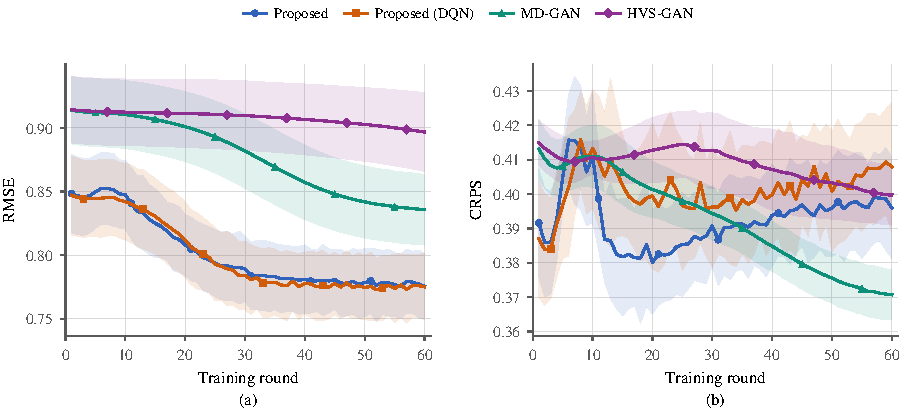
\includegraphics[width=\textwidth]{fig1_convergence.pdf}
\caption{Convergence against federated GAN baselines: (a) RMSE and (b) CRPS
versus training round, with 95\% confidence bands over five seeds.}
\label{fig:conv}
\end{figure*}

\begin{figure*}[!t]
\centering
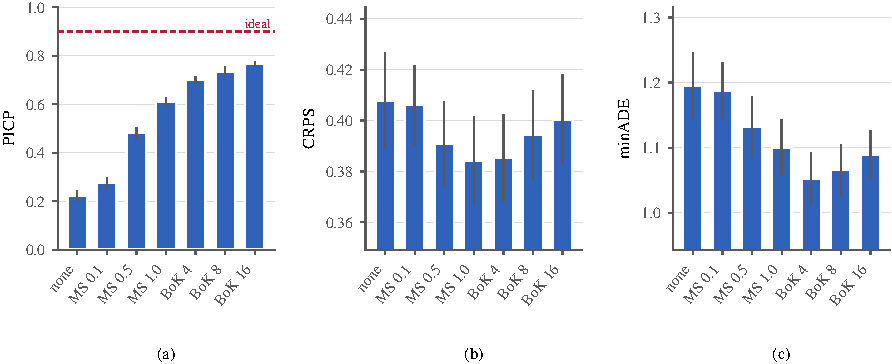
\includegraphics[width=\textwidth]{fig4_calibration.pdf}
\caption{Effect of the supervision mechanism on (a) interval calibration,
(b) CRPS and (c) minADE. Panels (b) and (c) use a non-zero baseline.}
\label{fig:calib}
\end{figure*}

\begin{figure*}[!t]
\centering
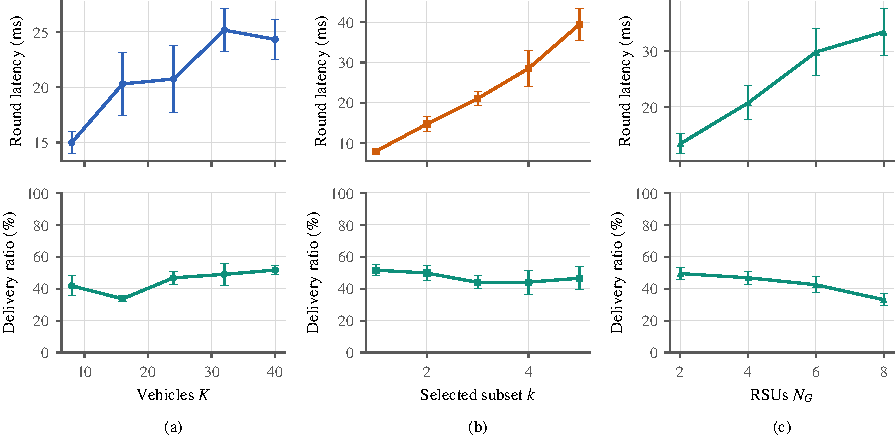
\includegraphics[width=\textwidth]{fig7_ns3_scalability.pdf}
\caption{Measured IEEE 802.11p behaviour of one synchronisation round: latency
(top) and delivery ratio (bottom) versus (a) vehicle count, (b) active subset
size and (c) RSU count, for a 600\,m deployment.}
\label{fig:ns3}
\end{figure*}

% =====================================================================
\begin{thebibliography}{99}
%% TODO: merge with the earlier submission's bibliography; only entries newly
%% required by this revision are listed.
\bibitem{arjovsky2017wgan}
M.~Arjovsky, S.~Chintala, and L.~Bottou, ``Wasserstein GAN,''
\emph{arXiv:1701.07875}, 2017.

\bibitem{hardy2019mdgan}
C.~Hardy, E.~Le~Merrer, and B.~Sericola, ``MD-GAN: Multi-discriminator
generative adversarial networks for distributed datasets,'' in \emph{Proc. IEEE
IPDPS}, 2019, pp.~866--877.

\bibitem{wu2024hvsgan}
L.~Wu, H.~Lin, and X.~Wang, ``Federated training generative adversarial networks
for heterogeneous vehicle scheduling in IoV,'' \emph{IEEE Internet Things J.},
2024.

\bibitem{gneiting2007crps}
T.~Gneiting and A.~E. Raftery, ``Strictly proper scoring rules, prediction, and
estimation,'' \emph{J. Amer. Statist. Assoc.}, vol.~102, no.~477, pp.~359--378,
2007.

\bibitem{creswell2018gan}
A.~Creswell \emph{et al.}, ``Generative adversarial networks: An overview,''
\emph{IEEE Signal Process. Mag.}, vol.~35, no.~1, pp.~53--65, 2018.
\end{thebibliography}

\end{document}
